\documentclass[12pt,a4paper]{article}
\usepackage{fontspec}
\usepackage{xunicode}
\usepackage{csquotes}
\usepackage{enumitem}
%\usepackage{titling}
\usepackage{setspace}
\usepackage{xcolor}
\usepackage[french]{babel}
\usepackage[style=enc]{biblatex}
\usepackage{graphicx}
\usepackage{pythonhighlight}
\usepackage{color}
\usepackage{listings}

\usepackage[hidelinks,linktoc=all]{hyperref}

\setlength{\parindent}{0pt}
\setlength\bibitemsep{1.5\itemsep}
\setlength{\footnotesep}{0.8\baselineskip}
\addtolength{\skip\footins}{1pc plus 5pt minus 3pt}

\renewcommand{\baselinestretch}{1.0} 

\definecolor{dkgreen}{rgb}{0,0.6,0}
\definecolor{gray}{rgb}{0.5,0.5,0.5}
\definecolor{mauve}{rgb}{0.58,0,0.82}
\definecolor{gray}{rgb}{0.4,0.4,0.4}
\definecolor{darkblue}{rgb}{0.0,0.0,0.6}
\definecolor{lightblue}{rgb}{0.0,0.0,0.9}
\definecolor{cyan}{rgb}{0.0,0.6,0.6}
\definecolor{darkred}{rgb}{0.6,0.0,0.0}


\lstset{
	basicstyle=\ttfamily\footnotesize,
	columns=fullflexible,
	showstringspaces=false,
	numbers=left,                   % where to put the line-numbers
	numberstyle=\tiny\color{gray},  % the style that is used for the line-numbers
	stepnumber=1,
	numbersep=5pt,                  % how far the line-numbers are from the code
	backgroundcolor=\color{white},      % choose the background color. You must add \usepackage{color}
	showspaces=false,               % show spaces adding particular underscores
	showstringspaces=false,         % underline spaces within strings
	showtabs=false,                 % show tabs within strings adding particular underscores
	frame=none,                   % adds a frame around the code
	rulecolor=\color{black},        % if not set, the frame-color may be changed on line-breaks within not-black text (e.g. commens (green here))
	tabsize=2,                      % sets default tabsize to 2 spaces
	captionpos=b,                   % sets the caption-position to bottom
	breaklines=true,                % sets automatic line breaking
	breakatwhitespace=false,        % sets if automatic breaks should only happen at whitespace
	title=\lstname,                   % show the filename of files included with \lstinputlisting;
	% also try caption instead of title  
	commentstyle=\color{gray}\upshape
}


\lstdefinelanguage{XML}
{
	morestring=[s][\color{mauve}]{"}{"},
	morestring=[s][\color{black}]{>}{<},
	morecomment=[s]{<?}{?>},
	morecomment=[s][\color{dkgreen}]{<!--}{-->},
	stringstyle=\color{black},
	identifierstyle=\color{lightblue},
	keywordstyle=\color{red},
	morekeywords={xmlns,xsi,noNamespaceSchemaLocation,type,id,x,y,source,target,version,tool,transRef,roleRef,objective,eventually}% list your attributes here
}

\begin{document}
	

%front page
\begin{center}
	
	\bigskip
	
	\begin{large}				
		ÉCOLE NATIONALE DES CHARTES\\
		UNIVERSITÉ PARIS, SCIENCES \& LETTRES
	\end{large}
	\begin{center}\rule{2cm}{0.02cm}\end{center}
	
	\bigskip
	\bigskip
	\bigskip
	\begin{large}
		Francesco Paolo Savatteri\\
		\vspace{1.3\baselineskip}
		Mai 2024
	\end{large}
	%selon le cas
	
	\vspace{8\baselineskip}
	
	\setstretch{1.5}
	\begin{Large}
		Encodage XML d'un forum Incel italien
	\end{Large}
	
	
	
	\vfill
	
	
\end{center}


\thispagestyle{empty}	
\cleardoublepage




\tableofcontents
\clearpage

\section{Source des données}
Les données encodées en XML proviennent du forum en ligne \emph{Il forum dei brutti}\footnote{“Le forum des moches” en italien}. Il s'agit de l'un des principaux espaces de discussion de la communauté Incel italienne. “Incel” est une contraction de “Involuntary Celibates” (célibataires involontaires) et désigne une communauté en ligne de personnes - principalement des hommes blancs hétérosexuels. \\

Le point commun des membres de cette communauté est que beaucoup d'entre eux ne parviennent pas à avoir des relations romantiques et sexuelles avec des femmes et ont des croyances fortement misogynes. \\ 
Les textes encodés sont en italien et n'ont pas été traduits en français. Ceci pour deux raisons. D'une part, il s'agit de considérations pratiques : il y a 96.000 messages encodés, pour un total de plus de 19 millions de caractères. D'autre part, le contenu de ces textes est très problématique, plein de messages haineux et, dans certains cas, même violents.\\

Les données ont été récupérées à l'aide de techniques de \emph{web scraping}.

\section{Encodage et requêtes}

Les publications au sein du forum sont divisées en \emph{threads}: des fils de discussion qui portent sur un certain sujet. Chaque fil de discussion contient un nombre variable de publications.

Les éléments que je souhaitais conserver dans l'encodage xml sont les suivants :
\begin{itemize}[label=•]
	\item titre des fils de discussion
	\item auteur des messages
	\item date et heure de publication
	\item texte des messages
\end{itemize}

Pour ce faire, j'ai créé la structure suivante: 
\newpage
\begin{center}
\begin{figure}[h!]
	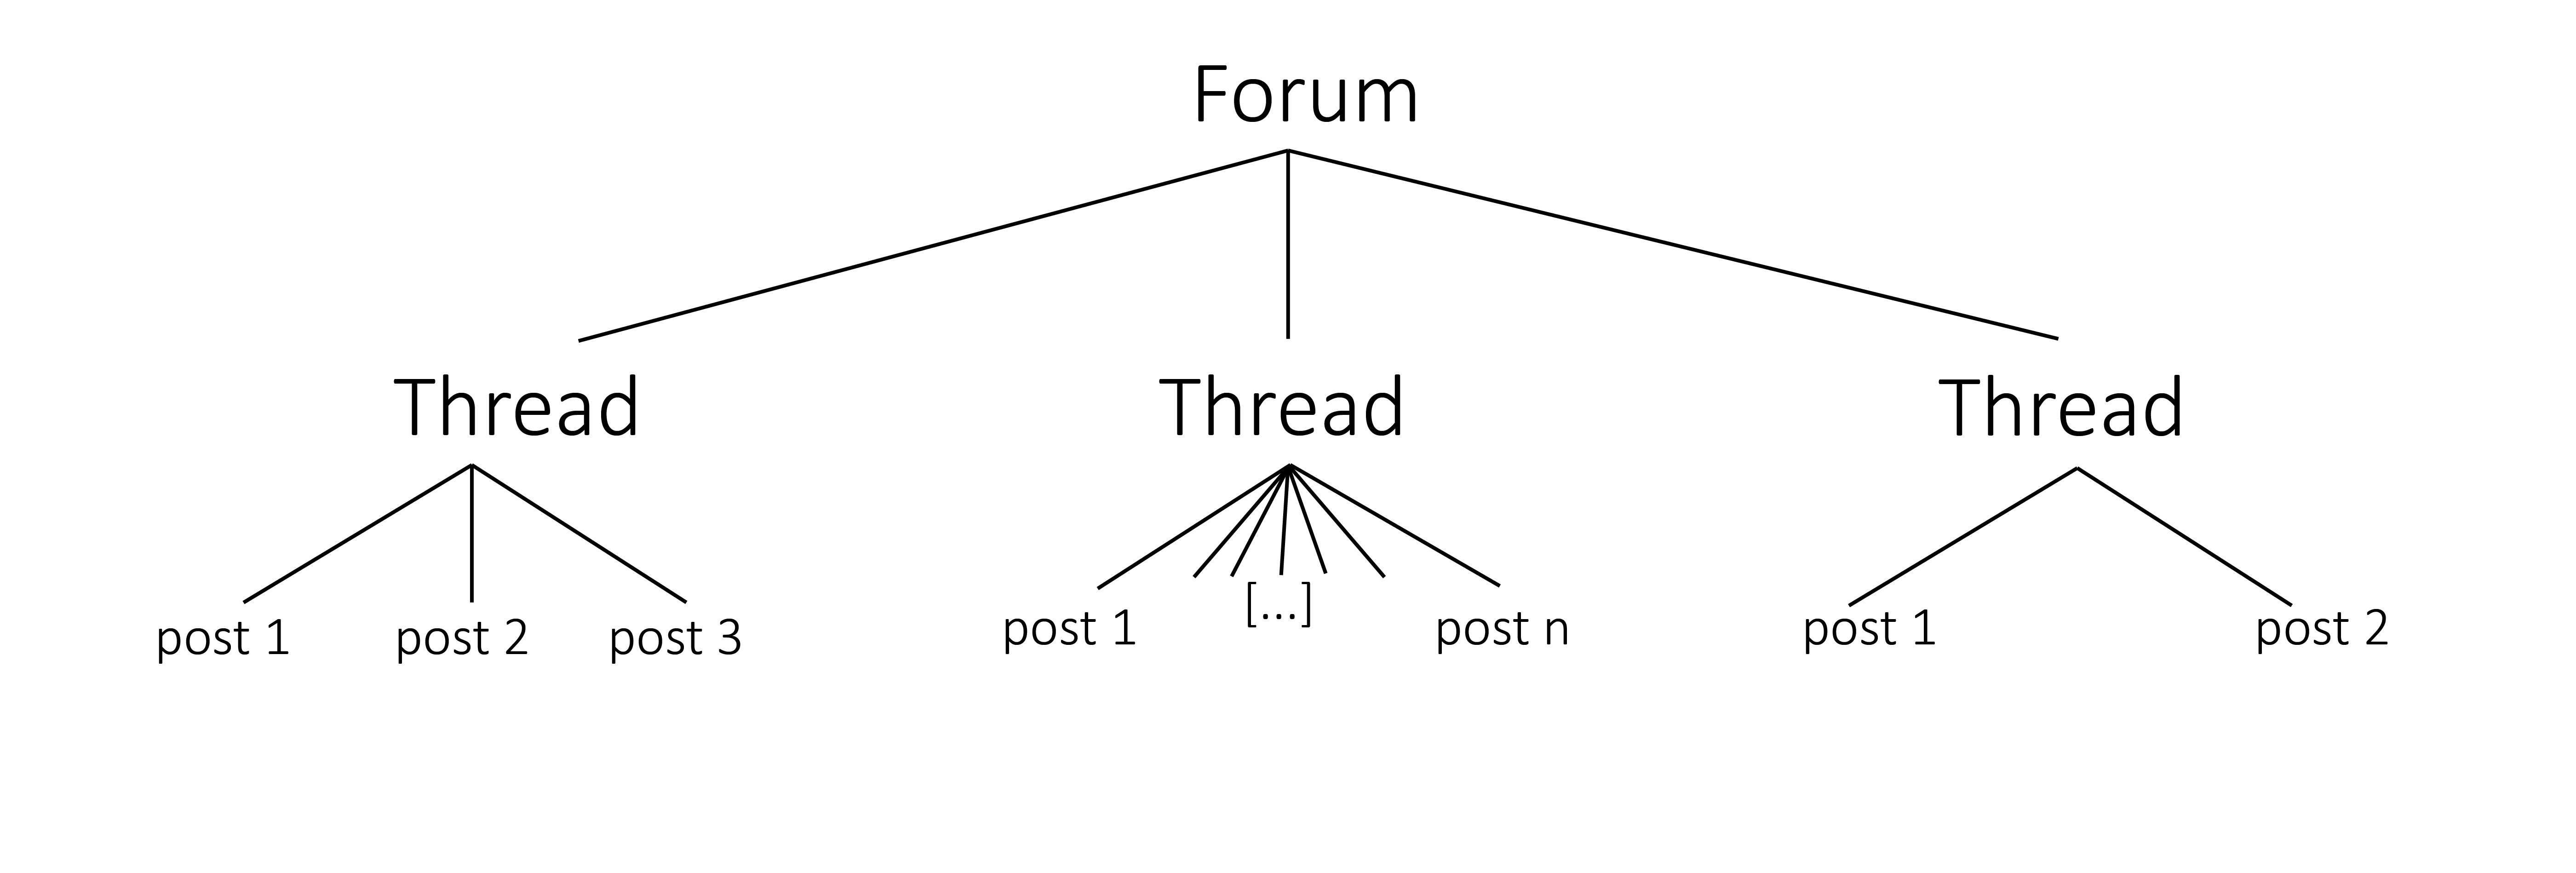
\includegraphics[scale=0.3,]{../../images/image_1.png}
\end{figure}
\end{center}

L'élément racine est donc <forum> et ensuite il y a les différents fils, marqués par l'élément <thread>. Chaque fil contient une quantité variable de publications sous la forme de <post>. Chaque <post> contient des informations sur l'auteur, la date et l'heure de publication, ainsi que le texte.

Voici un exemple de thread: \\

\begin{lstlisting}[language=XML]
	<thread title="Sondaggi">
	<post id="0">
	<date year="2023" month="12" day="11">2023-12-11</date>
	<time>13:36:59</time>
	<author who="#SanTan">SanTan</author>
	<text>Si possono fare i sondaggi qui?</text>
	</post>
	<post id="1">
	<date year="2023" month="12" day="11">2023-12-11</date>
	<time>13:43:25</time>
	<author who="#Ispettore_Derrick">Ispettore Derrick</author>
	<text>Me li chiedevo anche io ieri quando misi il mio simpatico sondaggio su Gino&amp;C</text>
	</post>
	<post id="2">
	<date year="2023" month="12" day="11">2023-12-11</date>
	<time>15:00:34</time>
	<author who="#bless123">bless123</author>
	<text>Non lo so ma non credo</text>
	</post>
	</thread>

\end{lstlisting}

Chaque post possède un élément « id » qui commence à 0 - pour le premier post d'un fil de discussion - et augmente d'une unité pour chaque nouveau element. Cela permet d'effectuer des recherches XPATH en fonction du nombre de post par fil de discussion.\\

Par exemple, dans la requête:
 \begin{lstlisting}
	//post[@id>9]/ancestor::thread/@title 
\end{lstlisting} 
On obtient les titres des thread qui ont plus de dix éléments <post>.\\

L'élément <date>, quant à lui, comprend les attributs année, jour et mois. Cela est très utile pour effectuer des requêtes XPATH en fonction du temps. Examinons les requêtes XPATH suivantes :\\

\begin{lstlisting}
	//post[./date/@month=12 and ./date/@year=2023]
	
	//date[@day=10]/ancestor::thread/@title
	
	for $x in distinct-values(//date/@month) 
	return concat((//date[@month=$x]/@year)[1], '/',$x, ' --->', count(//date[@month=$x]))
\end{lstlisting}

La première requête identifie tous les post publiés au cours du mois de décembre 2023. La deuxième identifie les titres de tous les fils de discussion dans lesquels il y a au moins un post publié le 10e jour d'un mois quelconque. La dernière requête, plus complexe, renvoie plutôt le nombre de post publiés chaque mois (les données couvrant une période allant d'octobre 2023 à avril 2024, il n'est pas nécessaire de travailler sur la distinction des différentes années). \\

L'attribut « who » des éléments <author> ne serait en fait pas strictement nécessaire, puisque les noms des auteurs sont toujours donnés de la même manière (contrairement, par exemple, aux noms des personnages d'un roman). Il s'agit donc plutôt d'un choix pour rendre les noms des auteurs plus visible et les requêtes XPATH plus claires.\\

L'encodage a été réalisé via un script python qui a transformé les données initialement en CSV en format XML. Cela a permis de transformer automatiquement une grande quantité de données. \\
Après la transformation, les données ont dû être nettoyées afin de rendre le format XML valide, notamment en ce qui concerne l'\emph{escaping} des caractères tels que « \& », « < » et « > » lorsqu'ils sont présents dans les textes des articles ou les noms des auteurs.

Le schéma RELAX NG généré automatiquement par le document XML a des règles très strictes à cause de la structure elle-même des données. Tous les éléments à l'interieur des <post> sont obligatoires, de même que tous les attributs des éléments. Les seuls éléments dont la quantité est variable (mais qui restent obligatoires) sont le <post> et le <thread>, qui dans le schéma sont marqués comme <oneOrMore>.

\section{Les feuilles de transformation}
La feuille de transformation que j'ai créée transforme le texte xml en un csv avec deux colonnes : le nom de l'auteur et le nombre d'articles. L'aspect le plus délicat a été de trouver un moyen d'itérer le comptage uniquement sur les valeurs uniques des noms d'auteurs, afin d'éviter les répétitions. Ceci a été réalisé en utilisant la fonction \emph{distinct-values()}.  Le problème, cependant, était d'obtenir un code qui ne produise pas d'erreurs de validation. En effet, dans plusieurs cas j'ai obtenu des erreurs de validation. Par exemple, le code suivant renvoie l'erreur suivante: \emph{The required item type of the first operand of '/' is node(), but the supplied expression {\$currentAuthor} has item type xs:anyAtomicType}.

\begin{lstlisting}[language=XML]
	<?xml version="1.0" encoding="UTF-8"?>
	<xsl:stylesheet xmlns:xsl="http://www.w3.org/1999/XSL/Transform"
	xmlns:xs="http://www.w3.org/2001/XMLSchema"
	exclude-result-prefixes="xs"
	version="2.0">
	<xsl:output method="text" />
	
	<xsl:template match="/">
	
	<xsl:text>author,number_of_posts&#10;</xsl:text>
	<xsl:for-each select="distinct-values(//author)">
	<xsl:variable name="currentAuthor" select='.'/>
	<xsl:value-of select="$currentAuthor/@who" />
	<xsl:text>,</xsl:text>
	<xsl:value-of select="count(//author/@who[.=$currentAuthor/@who])"/>
	</xsl:for-each>
	
	</xsl:template>
	</xsl:stylesheet>
\end{lstlisting}

La raison des erreurs est que la fonction \emph{distinct-values()} ne renvoie pas des nœuds mais des valeurs atomiques. Pour résoudre ces problèmes, j'ai dû créer la variable \$currentAuthor comme une copie de l'élément courant, et j'ai dû créer une autre variable pour l'élément racine de tout le document. Le code final XSLT que j'ai utilisé se trouve dans les fichiers.
\\
Comme la fonction \emph{distinct-values()} n'existe que dans la version 2.0 de XSLT, j'ai créé un code qui est également compatible avec la version 1.0. Les deux codes se trouvent dans les fichiers to\_csv\_v1.xsl et to\_csv\_v2.xsl. Le code pour la version 1.0 est très inefficace et prend plusieurs minutes (476 secondes pour la précision) pour effectuer la transformation. Une version plus efficace a été créée avec chatGPT et se trouve elle aussi dans les fichiers. 

\section{Limites du travail}
Comme il s'agit d'un fichier XML créé avec du code python, il n'arrive à encoder que des informations de base. Il faudrait utiliser des systèmes beaucoup plus sophistiqués pour pouvoir créer un encodage XML automatisé des textes contenus dans les post du forum, en fonction de leur signification.

\end{document}